\chapter{Implementierung}
\label{ch:implementierung}

Um das System zu implementieren und zu testen wurde bereits existierende Software und Bibliotheken verwendet die in ihrer Funktion und Anwendung im Projekt kurz erläutert werden sollen.


\section{Simulationsumgebung}
\subsection{Simulator CARLA}
Der gesamte Systeminput wird durch den CARLA Simulator\cite{Dosovitskiy17} erzeugt. Nach eigener Aussage ist die Motivation hinter dem Projekt die Demokratisierung in der Forschung und Entwicklung autonomen Fahrens. CARLA (Car learning to act) ist ein Open-Source Simulator basierend auf der Unreal Engine 4. Die Engine ist kostenlos für nicht-kommerzielle Nutzung und bietet eine Rendering, physikalische Modelle (PhysXVehicles) und NPC Logik für Fu{\ss}gänger und andere Verkehrsteilnehmer. CARLA startet als Server mit einer Python Client API. Über die API können Parameter der Simulation wie z.B. die Map oder das Wetter gesetzt werden. Ein gespawntes Fahrzeug ist ein Client der über Sockets mit dem Server kommuniziert. Die echte Position des Fahrzeugs wird über einen Ground Truth Pseudo-Sensor ausgegeben.


\subsection{ROS2 Framework für Prozesskommunikation}

\begin{figure}[h!]
	\centering
	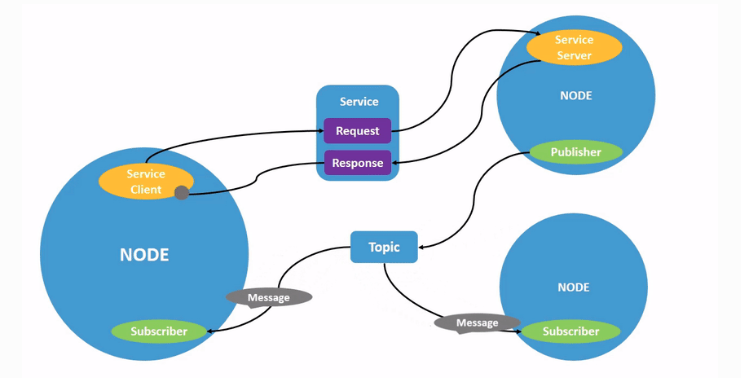
\includegraphics[width=0.8\textwidth]{pictures/06_ROS_nodes.png}
	\caption[ROS2 Node Netzwerk]{Ein ROS2 System besteht aus vielen Nodes die Nachrichten über eine Publish-Subscriber Architektur austauschen. (ROS2 Dokumentation, 2022)}
\end{figure}


Das Robot Operating System ROS2 wird seid 2007 entwickelt und besteht aus einer Sammlung von Bibliotheken und Tools für Robotik Anwendungen. Anders als der Name vermuten lässt, ist ROS2 kein in sich geschlossenes Betriebssystem sondern ein Framework das unter Linux betrieben werden kann. ROS2 und darin zur Verfügung stehenden Software sind Open Source.
\newline

In einem ROS2 System läuft jeder Prozess in einem Node. Ein Programm kann aus mehren Nodes bestehen aber ein Node sollte immer nur einen Zweck erfüllen. Dadurch werden die Systeme Modular und ein Node kann in unterschiedlichen Systemen eingesetzt werden. Bei der Initialisierung eines Nodes können Einstellungen durch sog. Parameter übergeben werden. Jeder Node verwaltet seine eigenen Parameter. Beispielsweise werden für die Stereo und RGB-D Odometrie zwei Nodes vom selben Modul mit unterschiedlicher Parametrierung instanziiert.
\newline

Alle Daten im ROS2 Netzwerk werden in ROS2 Message Datentypen gepackt. Die Nachrichten werden über ein Publish-Subscriber-Architektur im Netzwerk verteilt. Jeder Node kann beliebig viele Topics veröffentlichen oder abonnieren. Das Topic agiert als Datenbus des Systems.\newline 
Der gro{\ss}e Vorteil dieser Architektur ist die Einführung eines Standards für die Schnittstellen der Programme. Ohne Veränderung an dem Node für die Visuelle Odometrie vornehmen zu müssen, kann die Datenquelle geändert werden und es ist auch keine Kenntnis über die Empfänger der Daten nötig. Die Eingangdaten müssen nur vom Typ \textit{sensor\_msgs Image} und \textit{CameraInfo} sein und ein Empfänger der Odometrie Daten vom Typ \textit{nav\_msgs} \textit{Odometry} erwarten.

\subsection{Kameradaten}

\begin{figure}[!h]
  \begin{center}
    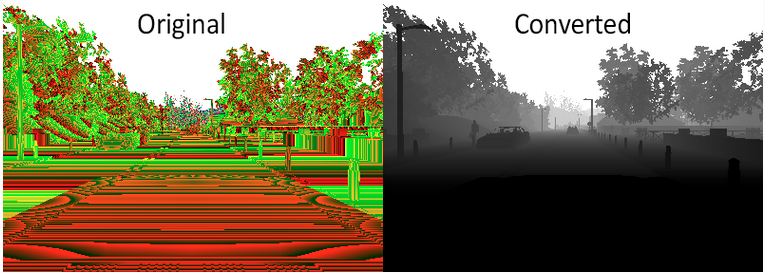
\includegraphics[width=0.75\textwidth]{pictures/depth_map_carla.png}
    \caption[CARLA Tiefenkarte]{Depth Map Pseudosensor des Simulators in Original und User freundlichen Konvertierung. (CARLA Dokumentation, 2022)}
  \end{center}
\end{figure}

Der Simulator verfügt viele, für autonomes Fahren relevante, Sensoren wie Kamera, Lidar, IMU, GNSS ect.. Die Sensoren werden über eine JSON-Konfigurationsdatei instanziiert und stehen immer in Relation zum Fahrzeug. Dabei sind alle Distanzen in Metern zu lesen.
\newline

Für die vorliegende Arbeit wurden zwei RGB Kamerasensoren zu einer Stereokamera konfiguriert und eine RGB Kamera mit Depth Map Sensor als RGB-D Kamera verwendet. Die Kameras müssen nicht rektifiziert werden und die intrinsischen (Kamera internen) Parameter sind direkt bekannt. Die Auswahl und Positionierung erfolgt über die CARLA API. Die Position wird dabei in Metern und immer in Bezug zum Fahrzeug definiert. Bilddaten werden vom Server als BGRA Bytearray gesendet.

Folgende Effekte aus dem Simulator haben Einfluss auf das Kamerabild:\\
\newline
\textit{Grain jitter} erzeugt ein künstliches Rauschen. \textit{Blooming} erzeugt eine helle Verzeichnung in der Umgebung einer Überbelichtung. \textit{Auto exposure} ändert den Bild-Gammawert, um Anpassung an dunklere oder hellere Bereiche zu simulieren. \textit{Lens flares} simuliert di Reflexion heller Objekte auf der Linse. \textit{Depth of field} lässt Objekte in der Nähe oder sehr weit von der Kamera unscharf werden. \newline


Unglücklicherweise werden diese Effekte über die Unreal Engine erzeugt und nicht in der Kamera in CARLA. Ein Blooming Effekt würde bei modernen CMOS beispielsweise i.d.R. nicht auftreten sondern ist ein CCD Phänomen. Auch die Implementierung des Auto-Exposure Effekts ist bei CARLA dem Menschlichen Auge nachempfunden um beim User einen besseres Optisches Erlebnis zu erzielen anstatt die Kamera korrekt zu modellieren.\newline


\subsection{Transformationsbaum}

\begin{figure}[h!]
  \centering
    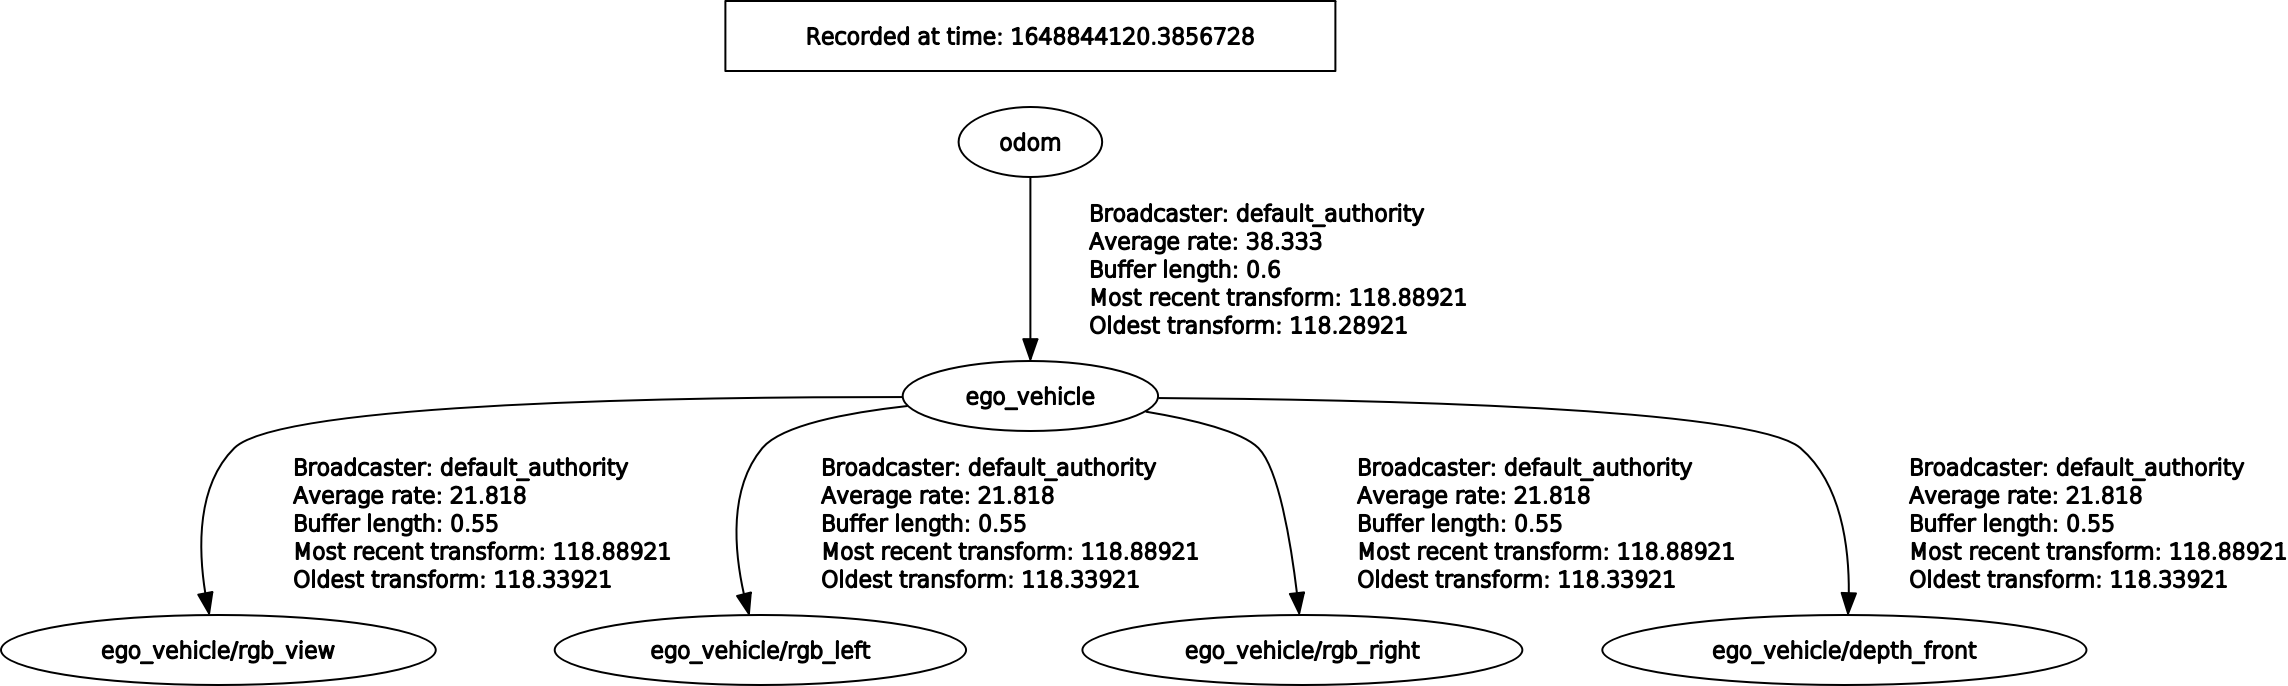
\includegraphics[width=0.75\textwidth]{pictures/05_tf_frames.png}
    \caption[ROS2 Transformationsbaum für Visuelle Odometrie]{ROS2 Transformationsbaum für den Versuchsaufbau.}
		\label{fig:tf}
\end{figure}

Im Netzwerk kann die räumliche Beziehung zwischen Nodes über einen Transformationsbaum abgebildet werden. Jeder Node hat sein eigenes Koordinatensystem. Über die Transformationen wird bekannt gegeben wie die Koordinatensysteme zu einander ausgerichtet sind. So kann beispielsweise definiert werden wo sich die Kameras in Bezug zum Mittelpunkt des Fahrzeugs befinden. Wird jetzt die Pose des Fahrzeugs aktualisiert, können auch alle Sensor Posen aktualisiert werden. 

Abbildung \ref{fig:tf} zeigt den Transformationsbaum des System. Neben den statischen Transformationen zwischen Sensoren und Fahrzeug (ego\_vehicle) ist auch die Transformation des Odometrie Frames zum Fahrzeug zu sehen. Wird das System in ein anderes Netzwerk eingebunden kann also über diesen Frame auf das Fahrzeug und alles was mit dem Fahrzeug verbunden ist lokalisiert werden.

\pagebreak
\section{Bibliotheken}

\subsection{Computer Vision Bibliothek OpenCV}

\begin{figure}[!h]
  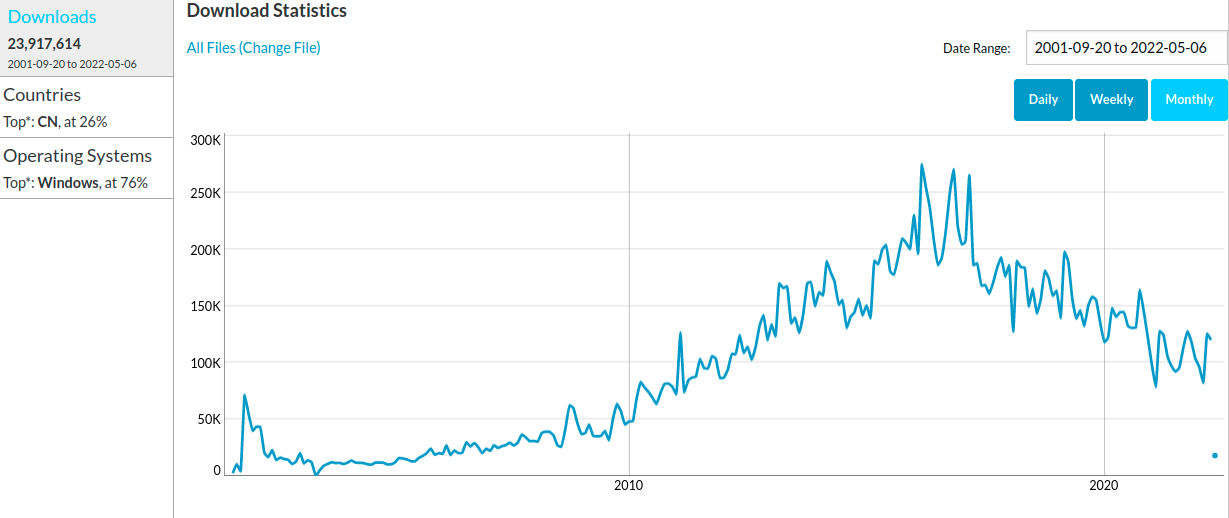
\includegraphics[width=0.9\textwidth]{pictures/06_cv_downloadstatistics.png}
  \caption[OpenCV Bibliothek Download Statistik]{SourceForge OpenCV Download Statistik zeigt über 23,9 Millionen Downloads seid dem 20.09.2001}
\end{figure}

Lokalisierung mittels Kameradaten ist ein bekanntes Problem der Bildverarbeitung. Über die Jahrzehnte sind viele Algorithmen und Funktionen entwickelt worden um die verschiedenen Aspekte der Problemstellung zu lösen. Über 2500 davon lassen sich in der Open Source Bibliothek OpenCV (Open Computer Vision) finden. OpenCV wurde ursprünglich von Intel entwickelt und hatte seine Erstveröffentlichung 2000. Der Fokus der Bibliothek liegt auf Echtzeit Bildverarbeitung. Viele Probleme der Bildverarbeitung sind äu{\ss}erst Rechenintensiv. Durch OpenCV sollen optimierte Implementierungen geschrieben werden und Robotik Ingenieure davon befreit 'das Rad neu erfinden zu müssen'.
\newline

OpenCV ist in C++ geschrieben bietet Interfaces in Python, Java, MATLAB und Mobile Device Ports. Durch die hohe Qualität der Bibliothek und die Fülle an Anwendungen der Bildverarbeitung wird OpenCV von sehr vielen Firmen und Forschungseinrichtungen benutzt wie beispielsweise Google, Microsoft, Sony, MIT, Intel, Siemens usw.. Die Zahl der Downloads liegt aktuell bei fast 24 Millionen.
\newline

Für den Systementwurf wurde OpenCV als Grundlage für das Prototyping verwendet. Die Bibliothek hat es ermöglicht einen schnellen praktischen Zugang zu der Theorie aus wissenschaftlichen Veröffentlichungen hinter der Bildverarbeitung zu erlangen. Stellenweise konnten Parameter für die VO heuristisch ermittelt werden und es erleichterte den Vergleich verschiedener Algorithmen.
\newline 

Neben der optimalen Implementierung von Algorithmen wird bei OpenCV auch an eigene Forschung zu neuen Methoden betrieben. Der im System verwendete ORB Algorithmus ist eine Eigenentwicklung der OpenCV Researcher. 
\newline

Alternativ zu OpenCV kann für das Prototyping beispielsweise MATLAB verwendet werden falls der Entwickler mit dieser Umgebung besser vertraut ist. Die Performance von MATLAB gegenüber OpenCV ist jedoch bis zu 80 mal langsamer \cite{cvmatlab}. Code der mit OpenCV geschrieben wurde kann zudem direkt auf dem Zielsystem laufen.

\subsection{V-SLAM Bibliothek RTAB-Map}
RTAB-Map ist eine standalone C++ Open Source Bibliothek für Real-Time Appearance Based Mapping. Unter der Verwendung von OpenCV werden RGB-D, Stereo and Lidar Graph-Based SLAM Algorithmen implementiert \cite{labbe}.
\newline

RTAB-Map wird auch als ROS und ROS2 Package veröffentlicht. Der ROS Philosophie folgend sind verschiedene Teiles der SLAM Algorithmen als Nodes implementiert, aus denen sich ein vollständiges SLAM zusammensetzt. Für Visual SLAM ist die visuelle Odometrie das Front-End zur Bildverarbeitung. Es gibt daher einen Stereo Odometrie Node aus RTAB-Map der zur Realisierung der visuellen Odometrie für die Fahrzeuge des CARS Projekt verwendet werden kann. \newline

Der Node hat eine Parameterliste von 242 Parametern die wie eine API für die unterliegenden Funktionen funktioniert. In den meisten Fällen sind die Parameter Übergabewerte an OpenCV Funktionen. Der Node bietet dadurch die Möglichkeit direkt eine VO Pipeline aufzurufen und sich vollständig auf die Parametrierung der CV Funktionen z.B. WindowSize der Merkmalsdetektoren zu konzentrieren.
